% id: 120-05
% book: 베이직쎈 확률과 통계 · 06 이항분포와 정규분포
% section: 실전 감각 UP
% figure: tikz:fig-120-05
% answer: 
% answer_source: 
% variant_level: 0 (원본 전사)
% 이 파일은 build.mjs 가 items.json 에서 만든다. 고칠 때는 items.json 을 고친다.
\smash{\raisebox{1.5mm}{\dmkichul{베이직쎈 확률과 통계 120쪽 05번}}}
\noindent\begin{minipage}[t]{0.58\linewidth}\vspace{0pt}\raggedright 어느 고등학교의 세 반 $\mathrm{A}$, $\mathrm{B}$, $\mathrm{C}$의 전체 학생 수는 같고, 세 반 학생들의 수학 수행 평가 점수는 각각 정규분포를 따른다. 세 반 $\mathrm{A}$, $\mathrm{B}$, $\mathrm{C}$의 수행 평가 점수의 정규분포곡선이 각각 위의 세 곡선 $\mathrm{A}$, $\mathrm{B}$, $\mathrm{C}$와 같을 때, 세 반 중 수행 평가 점수의 평균이 가장 낮은 반과 점수가 가장 고른 반을 차례대로 고르면?\end{minipage}\hfill\begin{minipage}[t]{0.4\linewidth}\vspace{0pt}\centering \resizebox{\ifdim\width>\linewidth\linewidth\else\width\fi}{!}{% 120-05(인쇄 120쪽) — 세 반 A, B, C 의 수행 평가 점수 정규분포곡선 세 개(가로축 x 하나 위에 겹쳐 그림).
% 스캔 화질이 낮아 TikZ 로 다시 그림. 곡선의 평균·산포는 원문 그림을 재어 맞췄다
% (A 가 가장 왼쪽, B 가 가장 높고 좁으며, C 가 가장 오른쪽이고 낮다). 라벨은 원문에 있는 A, B, C, x 뿐이고 눈금·평균값은 적지 않는다.
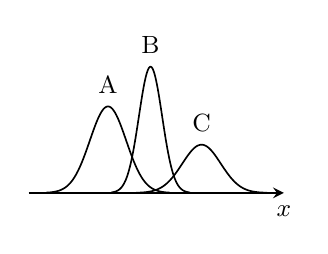
\begin{tikzpicture}[line width=0.6pt, x=0.36cm, y=0.36cm]
  \draw[->, >=stealth, line width=0.7pt] (-0.4,0) -- (8.6,0) node[below=1pt, font=\small] {$x$};
  \draw[domain=0.22:4.58, samples=120, smooth] plot (\x, {3.05*exp(-(\x-2.4)^2/(2*0.64*0.64))});
  \draw[domain=2.51:5.29, samples=120, smooth] plot (\x, {4.45*exp(-(\x-3.9)^2/(2*0.41*0.41))});
  \draw[domain=3.39:8.01, samples=120, smooth] plot (\x, {1.70*exp(-(\x-5.7)^2/(2*0.68*0.68))});
  \node[above=1pt, font=\small] at (2.4,3.05) {$\mathrm{A}$};
  \node[above=1pt, font=\small] at (3.9,4.45) {$\mathrm{B}$};
  \node[above=1pt, font=\small] at (5.7,1.70) {$\mathrm{C}$};
\end{tikzpicture}
}\end{minipage}\par
\begin{choices32}{$\mathrm{A}$, $\mathrm{B}$}{$\mathrm{A}$, $\mathrm{C}$}{$\mathrm{B}$, $\mathrm{A}$}{$\mathrm{B}$, $\mathrm{C}$}{$\mathrm{C}$, $\mathrm{B}$}\end{choices32}
